\section{Learning Significant Locations and Predicting User Movement With GPS}
This thesis by \cite{learning_significant_locations} from 2002 is one of the earliest contributions to present a system which uses GPS data to infer user context, and use this context. 

\subsection{Data Collection}
For data collection, a wearable GPS receiver was used which tracked user location during four months with an accuracy of 15 meters, meaning the same physical location may have resulted in slightly different GPS coordinates from day to day. For pre-processing data some of the data was discarded by setting the sensor to only log data while the user was travelling at a speed greater than 1 mile per hour, with the average human having a walking speed of about 3 miles per hour. 

\subsection{Finding Locations}
Given a data set of GPS points, a \textit{significant place} is found by examining data and finding periods of low user-movement. The duration of the period was (somewhat arbitrarily) chosen to be 10 minutes. Due to the 15 meter accuracy of the sensor, the location coordinates found may be somewhat noisy from day to day. In order to identify the mean of these noisy place locations, a modified version of the \textit{K-means} clustering algorithm was applied to the dataset, with a radius parameter. The optimal radius for the clustering algorithm is found by examining  the graph of the number of clusters found (K) as a function of the radius. The knee of the graph (see figure \ref{fig:knee-graph}) signifies the radius just before the number of locations begins to converge to the number of clusters found. This procedure effectively figures out which significant places belong to the same \textit{location} and which are outliers points which should be considered noise, i.e. they either do not belong to a location or there is too low confidence to say whether they do or not. 

\begin{figure}
    \centering
    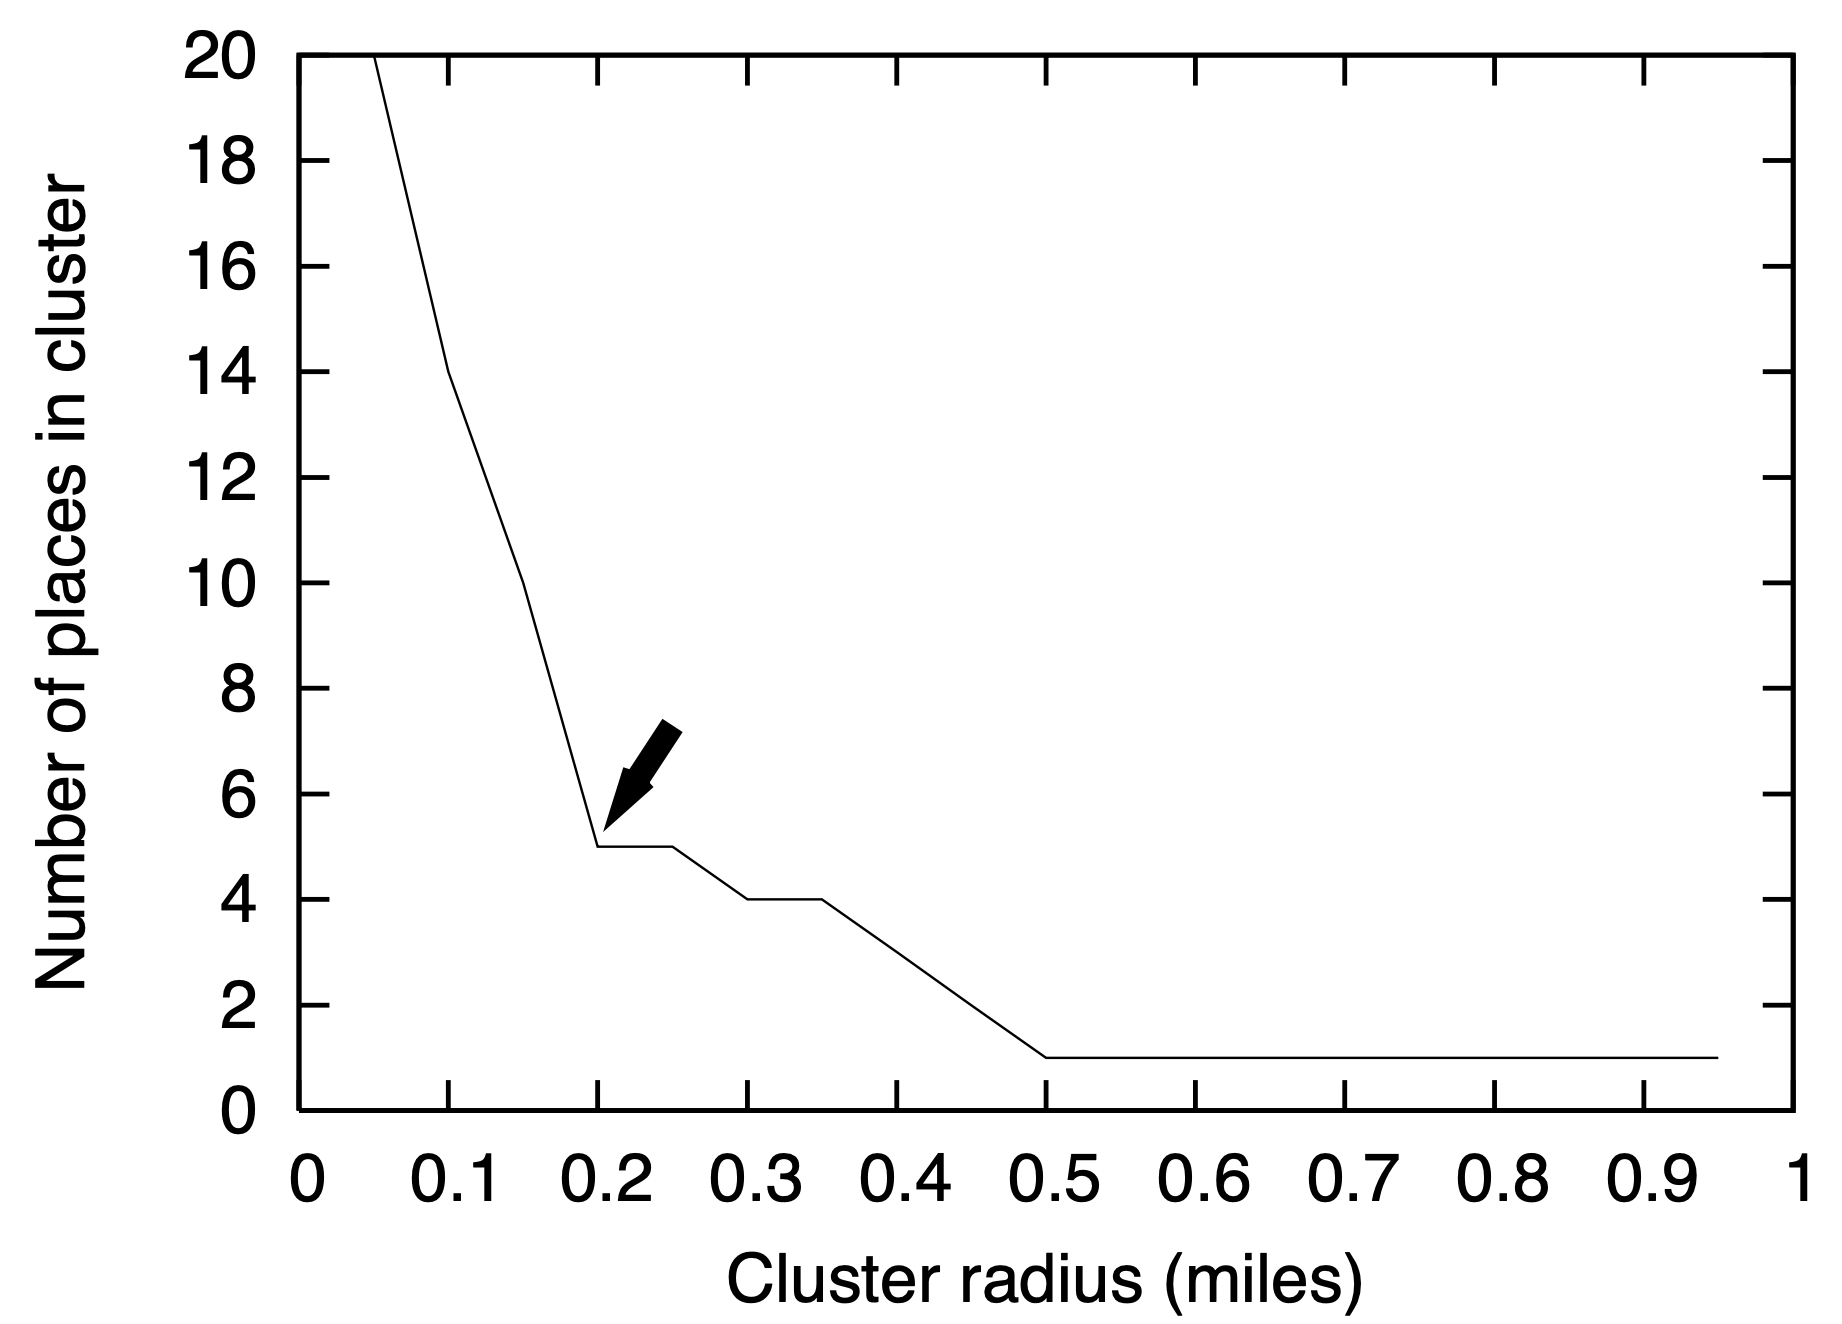
\includegraphics[width=0.5\textwidth]{images/knee_graph.png}
    \caption{The number of places found in the dataset the location radius parameter changes. The arrow indicates the knee in the graph at which point the radius will be used to find \textit{sub-locations}. Source \cite{learning_significant_locations}}
    \label{fig:my_label}
\end{figure}

\subsection{Finding Sub-locations}
Within a location, several \textit{sub-locations} may exists, which are perhaps best exemplified by a university campus, as a location, having several buildings for different departments, i.e. \textit{sub-locations}. To find these, all \textit{significant place} data-points belonging to a \textit{location} is given as input to previously described clustering algorithm. The optimal radius is once again found by looking at the knee on the graph and from this optimal parameter choice, the \textit{sub-locations} within a given location are identified.

\subsection{Prediction}
A Markov model was set up with each state representing a Location and transitions representing real-life transitions between locations. To compute the probability of a path, or a transition between places, the relative frequency of the path was computed.

